\documentclass[11pt]{article}
\usepackage{theme}
\usepackage{shortcuts}
\usepackage{bm}
\usepackage{subcaption}
\usepackage{graphicx}
\usepackage{algorithm}
\usepackage{algpseudocode}

\title{Mini-Project (ML for Time Series) - MVA 2023/2024 \\ \Large{\textit{Time warp invariant kSVD:\\ Sparse coding and dictionary learning for time series under time warp}}}

\author{
Manal Akhannouss \email{manal.akhannouss@eleves.enpc.fr} \\
Alexandre Lutt \email{alexandre.lutt@eleves.enpc.fr}
}

\begin{document}
\maketitle

\section{Introduction and contributions}

\paragraph{} In this project, we aim to provide an open-source implementation of the Time Wrap Invariant Orthogonal Matching Pursuit and Time Wrap Invariant-kSVD algorithms introduced in \cite{main_paper}, and to reproduce some of the experimental results of the original paper. 

The classical sparse coding and dictionary learning such as Orthogonal Matching Pursuit (OMP) and kSVD have been widely used in the field of time series analysis. However, these methods are not robust to time warp, which is a common phenomenon in time series. This led the authors of \cite{main_paper} to propose new sparse coding and dictionary learning algorithms that are robust to time warp and allow using variable-length time series. The original paper introduces two algorithms, Time Warp Invariant Orthogonal Matching Pursuit (TWI-OMP) and Time Warp Invariant kSVD (TWI-kSVD). The main idea behind these algorithms is to use a dynamic programming approach to compute the optimal alignment between the atoms of the dictionary and the samples.

During this project, we decided to split the work in two parts. First, Alexandre implemented the different algorithms, then Manal ran experiments to try to reproduce the claimed results. It is worth noting that no codebase was provided by the authors, and that we had to implement everything from scratch. Our joined experiments and tests also led us to propose a new classification strategy to challenge the original one. We also had to make some assumptions regarding the implementation of the algorithms, as well as the preprocessing of the datasets, as many methodological steps were omitted in the paper. Mainly, we had to make assumptions regarding the preprocessing, the size of atoms in dictionaries, and dictionaries initialization. We will discuss these assumptions in more details in the following sections.

\section{Method}

\subsection{Sparse coding}

\paragraph{} Sparse coding is a method that allows to represent a signal as a linear combination of a few elements of a dictionary. This problem is usually solved with a matching pursuit \cite{matching_pursuit} algorithm such as Orthogonal Matching Pursuit \cite{orthogonal_matching_pursuit} (OMP), which is a greedy algorithm that allows to find the sparse code of a signal by iteratively selecting the atom of the dictionary that is the most correlated with the residual.

\paragraph{Time Warp Invariant Orthogonal Matching Pursuit} is a variant of the OMP algorithm \cite{orthogonal_matching_pursuit} that allows to find the sparse code of a signal by iteratively selecting the atom of the dictionary that is the most correlated with the residual, after having computed the optimal alignment between the atoms and the residual. More precisely, the algorithm aims to solve the following:
\begin{alignat*}{4}
    \min_{\bm{\alpha}, \bm{\Delta}} &\quad \norm{\bm{x} - \sum \limits_{j=1}^K \alpha_j \bm{\Delta_j} \bm{d_j}}_2^2 \tag{TWI Sparse Coding Problem} \\ 
    \text{s.t.} &\quad \norm{\bm{\alpha}}_0 \leqslant \tau \\
    &\quad  \bm{\Delta}_j \bm{1}_{p_j} = \bm{1}_q \text{, } \bm{\Delta}_j \in \{ 0, 1 \}^{q \times p_j} &\quad \forall j \in \{1, ..., K\}
\end{alignat*}
where $\bm{\Delta}_j$ is the optimal alignment matrix between the $j$-th atom of the dictionary and $\bm{x}$, $\bm{d}_j$ is the $j$-th atom of the dictionary, $p_j$ is the length of the $j$-th atom of the dictionary, $q$ is the length of $\bm{x}$, and $\bm{1}_n$ is a vector of size $n$ filled with ones. In what follows, we will often use the notation $\bm{d}_j^s = \bm{\Delta}_j \bm{d}_j$ to denote the modified $j$-th atom of the dictionary that is aligned with $\bm{x}$.

In order to obtain the optimal alignment matrix $\bm{\Delta}_j$, the authors of \cite{main_paper} proposed to use a dynamic programming approach to maximise the absolute cosine similarity between the $j$-th atom of the dictionary and the sample. The optimal alignment matrix between two vectors $\bm{x}$ and $\bm{y}$ is found by finding the minimal cost path in a cost matrix $\bm{C}$, where each element $c_{i, j}$ corresponds to the cosine similarity between the subseries aligned to maximise the cosine similarity. More precisely, $c_{i, j} = \dfrac{\langle \bm{x}_{i, j} \bm{y}_{i, j} \rangle}{\norm{\bm{x}_{i, j}}_2\norm{\bm{y}_{i, j}}_2} = f(M_{i, j})$, where $M_{i, j} = (\langle \bm{x}_{i, j} \bm{y}_{i, j} \rangle, \norm{\bm{x}_{i, j}}^2_2, \norm{\bm{y}_{i, j}}^2_2)$ is computed recursively:
\begin{alignat*}{3}
    M_{i, j} &= \begin{cases}
        (\langle \bm{x}_1 \bm{y}_1 \rangle, \norm{\bm{x}_1}^2_2, \norm{\bm{y}_1}^2_2) &\quad \text{if } i = 1 \text{ and } j = 1 \\
        (\langle \bm{x}_{i-1, 1} \bm{y}_{i-1, 1} \rangle + \bm{x}_i\bm{y}_1, \norm{\bm{x}_{i-1, 1}}^2_2 + \bm{x}_i^2, \norm{\bm{y}_{i-1, 1}}^2_2 + \bm{y}_1^2) &\quad \text{if } i > 1 \text{ and } j = 1 \\
        (\langle \bm{x}_{1, j-1} \bm{y}_{1, j-1} \rangle + \bm{x}_1\bm{y}_j, \norm{\bm{x}_{1, j-1}}^2_2 + \bm{x}_1^2, \norm{\bm{y}_{1, j-1}}^2_2 + \bm{y}_j^2) &\quad \text{if } i = 1 \text{ and } j > 1 \\
        f(\argmax (M_{i-1, j}, M_{i, j-1}, M_{i-1, j-1})) &\quad \text{if } i > 1 \text{ and } j > 1
    \end{cases}
\end{alignat*}
This method is very similar to the DTW algorithm, in the sense that it finds the optimal monotonically increasing alignment that matches beginnings and ends of series together, and computes the optimal alignment matrix between two signals of lengths $T_x$ and $T_y$ in $\mathcal{O}(T_x T_y)$ time. For more details, we refer the reader to Algorithm \ref{alg:twi_omp} and \cite{main_paper}. 

\subsection{Dictionary Learning}

\paragraph{} Dictionary learning is a method that allows to learn a dictionary from a set of signals $\bm{X}$, as well as the optimal assignments for each signal. The goal of dictionary learning is to find the best dictionary that can represent all signals. We can solve this problem using the kSVD algorithm \cite{ksvd}, which is an iterative procedure that aims to learn a dictionary of fixed size by alterning between dictionary updates and sparse coding using the SVD decomposition of the residuals. The global time complexity per iteration of this algorithm is in $\mathcal{O}(T N K \tau)$, where $T$ is the length of a time series.

\paragraph{Time Warp Invariant kSVD} is similar to kSVD, but it uses the TWI-OMP algorithm instead of the OMP algorithm to compute the sparse codes. Moreover, the update rule on the atoms and assignments is also changed. 

The main idea is to compute the residual errors $\bm{e}_i$ for each sample $\bm{x}_i$ that uses the $k$-th atom $\bm{d}_k$. We then update $\bm{d}_k$ using SVD on the rotated residuals $\bm{\varphi(\bm{e}_i)}$. The rotation is done using the rotation operator $\text{rotation}(\bm{a}, \bm{c}, \bm{c})$, which rotates $\bm{a}$ so that $\theta_{\hat{a}, c} = \theta_{a, b}$. In this case, $\bm{\varphi(\bm{e}_i)} = \text{rotation}(\bm{\Delta}_{i, k}^T\bm{e}_i, \bm{\Delta}_{i, k}^T\bm{d}_k^{s_i}, \bm{d}_k)$. Finally, we apply the reverse transformation to update $\bm{d}_k^{s_i}$ and $\bm{\alpha}_{i, k}$. The time complexity per iteration of this algorithm is in $\mathcal{O}(T^2 N K \tau)$, where $T$ is the maximum length. More details are provided in Algorithm \ref{alg:twi_ksvd} and \cite{main_thesis}.

\subsection{Evaluation metrics}

\paragraph{Original classification method} In the original paper, the authors proposed a classification method based on the reconstruction error. More precisely, they proposed to classify a sample $\bm{x}$ by encoding it using the concatenation of all the class dictionaries, and then by assigning it to the class that gives the lowest reconstruction error. This works under the assumption that only the adequate class atoms will be used to reconstruct the sample with a low reconstruction error. However, if the class atoms are close to each other, this method might not be able to classify the sample correctly.

\paragraph{Proposed classification method} During our experiments, we found that we could easily outperform the original classification method by encoding the sample $\bm{x}$ with each class dictionary separately, and then by assigning it to the class that gives the lowest reconstruction error. We will compare both approaches in the following sections.

\section{Data}

\subsection{Preprocessing}

\paragraph{} Regarding our data, we used the only two datasets of the original paper that were available online, BME (artificial univariate dataset) and DIGITS (MNIST-like dataset of handwritten digits). As mentioned in the introduction, many details were omitted in the original paper, which led us to make some assumptions regarding the preprocessing of the datasets. 

The first step of preprocessing has been to filter out series of the DIGITS dataset that were too long (more than 120 points) or too short (less than 80 points). The main reason behind it was to keep a reasonable computational time, as the TWI-OMP algorithm is quite slow. For the same reason, we preprocessed the BME and DIGITS datasets by respectively downsampling the series to 64 (instead of 128) and 40 to 60 points. Again, in order to keep runtimes reasonable, we decided to respectively keep 10 and 20 series of each class of each dataset for the train and test sets. The last step of our preprocessing has been to standardize the series to the $[-1, 1]$ interval. This was important to ensure that the series were comparable, and that the learned dictionaries would not be biased by the scale of the series.
    
\subsection{Datasets}

\paragraph{BME} This synthetic dataset consists in univariate time series of fixed size, with 3 balanced classes. The B (Begin) class contains sample with a positive jump at the beginning, the M (Middle) class contains samples without jumps, and the E (End) class contains samples with a positive jump at the end. Samples of each class are shown in Figure \ref{fig:BME_samples}.

\paragraph{DIGITS} This real-world dataset is composed of 2D time series of variable size with 10 balanced classes corresponding to digits handwritten on a digital screen. Samples are shown in Figure \ref{fig:DIGITS_samples}.

\subsection{Experimental setup}

\paragraph{} Before running the experiments, we had to make some other assumptions regarding the initialization of the dictionaries. Since the original paper only mentioned their lengths (10), we still had to figure out the size of the different atoms, as well as the way to initialize them. After a lot of trial and error, we decided to initialize the atoms of the dictionaries with random contiguous subsequences of samples from the training set, with a length equal to two thirds of the original sample length. When using the kSVD algorithm (which requires atoms of the same size as the samples), we simply used consistent positional zero padding.

Moreover, we kept the same methodological choices as in the original paper, which means we learned one dictionary per class on each dataset, using sparsity levels of 2, 5 and 10. We also used a number of iterations for the kSVD and TWI-kSVD algorithms that were consistent with the claims of the paper, which led us to use 10 iterations for each dataset. In order to fully use the time-warp invariance of the TWI-OMP algorithm, we did not restrict the window size when computing the optimal alignment between the atoms and the samples, at the cost of very long runtimes.

\section{Results}

\subsection{BME Dataset}

\paragraph{} First, let's have a look at a comparative example on Figure \ref{tab:1D_example}, where the same sample, has been reconstructed by both algorithms. There, we can see that the TWI-kSVD algorithm is able to reconstruct the sample with a lower reconstruction error at each sparsity level. 

When we look at the reconstruction errors of both algorithms on the BME dataset in Table \ref{tab:reconstruction_results_BME}, we can see that our implementation of the TWI-kSVD algorithm is able to reproduce the results of the original paper to some extent, in the sense that it gives a lower reconstruction error than the kSVD algorithm for all sparsity levels. However, the classification errors in Table \ref{tab:classif_results_BME} show that our implementation of kSVD gives a lower classification error than expected, whereas TWI-kSVD gives a classification error that is way higher than in the original paper, no matter the classification strategy. This could be due to the assumptions we made regarding the preprocessing of the dataset and the initialization of the dictionaries, but after trying many different approaches (no subsampling, different initialization strategies, etc...), we have not been able to reproduce the results of the original paper, which led us to question the reproducibility of the results. Contacting the authors also did not help, as we did not receive any answer.

\begin{table*}[!ht]
    \centering
        \begin{tabular}{ccc}
            \toprule
            \textbf{Sparsity/Models} & \textbf{kSVD} & \textbf{TWI-kSVD} \\
            \midrule
            \textbf{2} & $0.25551$ & $0.17313$ \\
            \textbf{5} & $0.19873$ & $0.12301$ \\
            \textbf{10} & $\bm{0.15060}$ & $\bm{0.08559}$ \\
            \bottomrule
        \end{tabular}
    \caption{Reconstruction $L_2$ errors on the BME dataset (lower is better)}
    \label{tab:reconstruction_results_BME}
\end{table*}

This is confirmed by the analysis of the reconstruction loss presented in Figure \ref{fig:loss_BME}. Indeed, we can see that the reconstruction loss of the TWI-kSVD algorithm is not decreasing as fast as the one of the kSVD algorithm, which might explain the higher classification error. We also tried to visualize the learned dictionaries as shown in Figure \ref{fig:learn_dicts_BME}. 

We also observe in Table \ref{tab:classif_results_BME} that our classification strategy provides a much lower classification error than the original one for the kSVD algorithm, but not for the TWI-kSVD algorithm. Our interpretation for the performance gap of the TWI-kSVD between our implementation and the original paper is that both classification criteria are based on the fact that the error reconstruction is lower for the correct class than for the other classes. However, as we can see in Figure \ref{fig:barplots}, the average reconstruction error is not the same for each class, which might explain the higher classification error.

\begin{table*}[!ht]
    \begin{minipage}{.55\linewidth}
      \centering
        \begin{tabular}{ccc}
            \toprule
            \textbf{Sparsity/Models} & \textbf{kSVD} & \textbf{TWI-kSVD} \\
            \midrule
            \textbf{2} & $\bm{0.22}$ & $0.58$ \\
            \textbf{5} & $0.30$ & $0.58$ \\
            \textbf{10} & $0.45$ & $\bm{0.47}$ \\
            \bottomrule
        \end{tabular}
        \caption*{Original classification strategy}
    \end{minipage}
    \begin{minipage}{.35\linewidth}
      \centering
        \begin{tabular}{ccc}
            \toprule
            \textbf{Sparsity/Models} & \textbf{kSVD} & \textbf{TWI-kSVD} \\
            \midrule
            \textbf{2} & $\bm{0.07}$ & $\bm{0.53}$ \\
            \textbf{5} & $0.08$ & $\bm{0.53}$ \\
            \textbf{10} & $0.10$ & $0.62$ \\
            \bottomrule
        \end{tabular}
        \caption*{Our classification strategy}
    \end{minipage} 
    \caption{Classification error rates on the BME dataset (lower is better)}
    \label{tab:classif_results_BME}
\end{table*}

\subsection{DIGITS Dataset}

\paragraph{} Now, let's have a look at a comparative example on Figure \ref{tab:2D_example}, where the same sample is reconstructed by both algorithms. We see that TWI-kSVD is able to reconstruct the sample with a lower sparsity level than kSVD, and overall with a lower reconstruction error.

Table \ref{tab:reconstruction_results_DIGITS} shows a higher reconstruction error with TWI-kSVD, which is the opposite of what was observed on the BME dataset and claimed in the original paper. We think this comes from the complexity of the dataset, and that TWI-kSVD is not able to learn a good dictionary, as shown in Figure \ref{fig:learn_dicts_DIGITS}.

\begin{table*}[!ht]
    \centering
        \begin{tabular}{ccc}
            \toprule
            \textbf{Sparsity/Models} & \textbf{kSVD} & \textbf{TWI-kSVD} \\
            \midrule
            \textbf{2} & $0.50133$ & $0.53786$ \\
            \textbf{5} & $0.30436$ & $0.32883$ \\
            \textbf{10} & $\bm{0.20911}$ & $\bm{0.21764}$ \\
            \bottomrule
        \end{tabular}
    \caption{Reconstruction $L_2$ errors on the DIGITS dataset (lower is better)}
    \label{tab:reconstruction_results_DIGITS}
\end{table*}

Regarding the classification errors, we still observe a great performance gap between our implementation and the original paper, as shown in Table \ref{tab:classif_results_DIGITS}. However, we observe that our classification strategy provides a lower classification error, at least for the kSVD algorithm.

\begin{table*}[!ht]
    \begin{minipage}{.55\linewidth}
      \centering
        \begin{tabular}{ccc}
            \toprule
            \textbf{Sparsity/Models} & \textbf{kSVD} & \textbf{TWI-kSVD} \\
            \midrule
            \textbf{2} & $\bm{0.27}$ & $0.73$ \\
            \textbf{5} & $0.53$ & $\bm{0.66}$ \\
            \textbf{10} & $0.63$ & $0.92$ \\
            \bottomrule
        \end{tabular}
        \caption*{Original classification strategy}
    \end{minipage}
    \begin{minipage}{.35\linewidth}
      \centering
        \begin{tabular}{ccc}
            \toprule
            \textbf{Sparsity/Models} & \textbf{kSVD} & \textbf{TWI-kSVD} \\
            \midrule
            \textbf{2} & $\bm{0.14}$ & $0.81$ \\
            \textbf{5} & $0.27$ & $\bm{0.76}$ \\
            \textbf{10} & $0.29$ & $0.88$ \\
            \bottomrule
        \end{tabular}
        \caption*{Our classification strategy}
    \end{minipage} 
    \caption{Classification error rates on the DIGITS dataset (lower is better)}
    \label{tab:classif_results_DIGITS}
\end{table*}

\newpage

{\small
\bibliographystyle{acm}
\bibliography{biblio}
}

\section{Appendix}

\paragraph{}

\begin{figure*}[!ht]
    \centering
    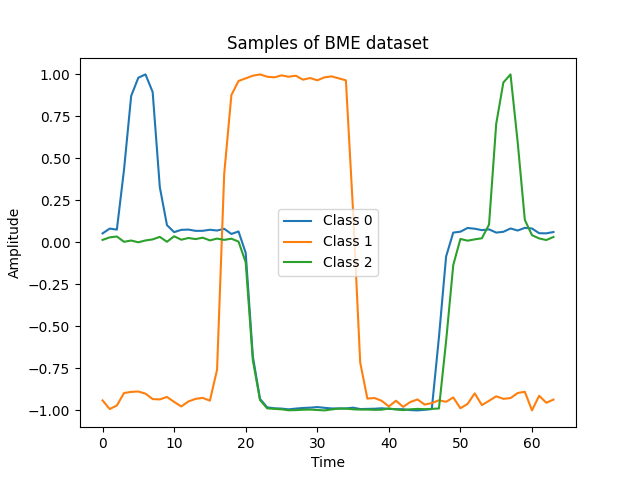
\includegraphics[scale=0.6]{../../figures/BME_samples.png}
    \caption{Samples of each class of the BME dataset} \label{fig:BME_samples}
\end{figure*}

\begin{figure*}[!ht]
    \centering
    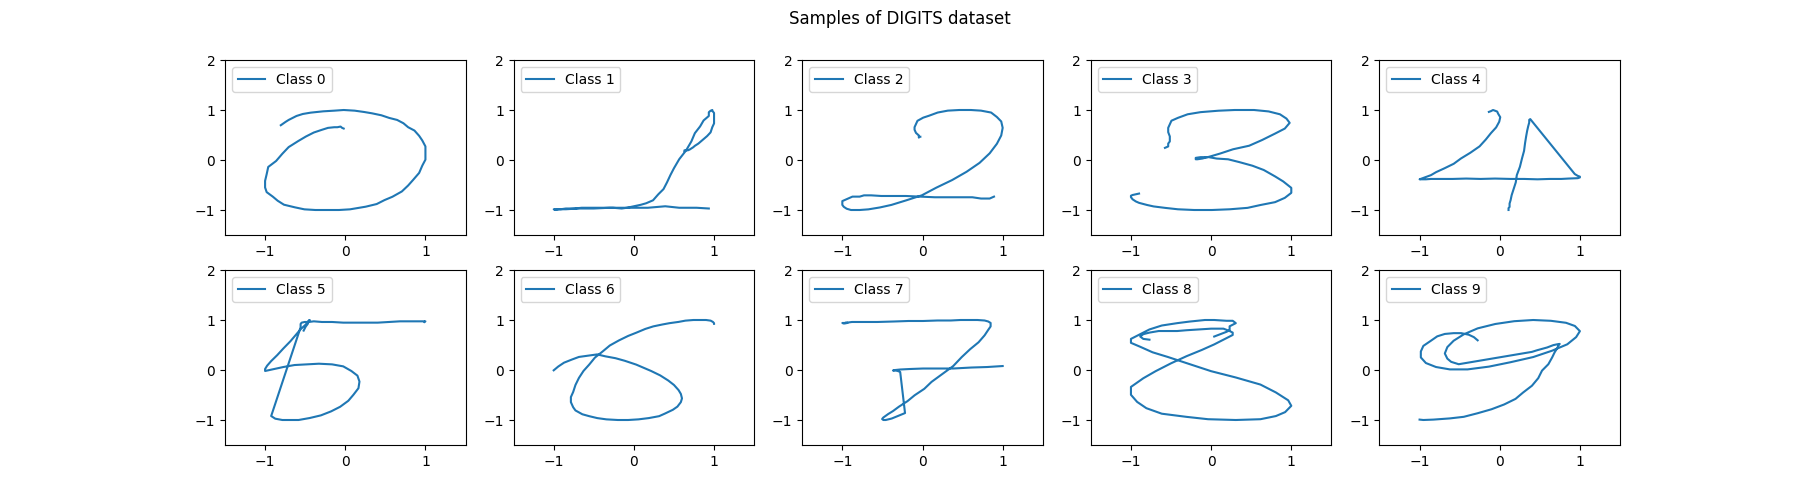
\includegraphics[scale=1.1]{../../figures/DIGITS_samples.png}
    \caption{Samples of each class of the DIGITS dataset} \label{fig:DIGITS_samples}
\end{figure*}

\begin{algorithm}
    \caption{TWI-OMP algorithm}\label{alg:twi_omp}
    \begin{algorithmic}
    \Require $\bm{x}, \bm{D}, \tau$
    \State $\bm{r} = \bm{x}$, $\Omega = \emptyset$
    \For{$t \in \{ 1, ..., \tau \}$}
        \State For all $k \notin \Omega$, compute $\bm{\Delta}_k$ and $C_k = \text{cosine}(\bm{x}, \bm{d_k})$ using dynamic programming
        \State $j = \argmax_{k \notin \Omega} C_k$
        \State $\Omega = \Omega \cup \{ j \}$, $\bm{S}_{\Omega} = (\bm{d_j^s})_{j \in \Omega}$
        \State $\bm{\alpha}_{\Omega} = \argmin_{\bm{\alpha}} \norm{\bm{x} - \bm{S}_{\Omega}\bm{\alpha}}_2$
        \State $\bm{x} = \bm{x} - \bm{S}_{\Omega} \bm{\alpha}_{\Omega}$
    \EndFor
    \State \Return $\bm{\alpha}_{\Omega}, \bm{\Delta} = (\bm{\Delta_k})_{k \in \Omega}$
    \end{algorithmic}
\end{algorithm}

\begin{algorithm}
    \caption{TWI-kSVD algorithm}\label{alg:twi_ksvd}
    \begin{algorithmic}
    \Require $\bm{X}, \bm{D}, \tau$
    \For{$t \in \{ 1, ..., n_{\text{iter}} \}$}
        \For{$i \in \{ 1, ..., N\}$}
            \State $\bm{\alpha}_i, (\bm{\Delta_{i, k}})_{k=1}^K = \text{TWI\_OMP}(\bm{x}_i, \bm{D}, \tau)$
        \EndFor
        \For{$k \in \{ 1, ..., K\}$}
            \State $\omega_k = \{ i \in \{ 1, ..., N\} : \bm{\alpha}_{i, k} \neq 0 \}$
            \State $\bm{E_k} = [\bm{e}_i]_{i \in \omega_k}$
            \State $\bm{\tilde{E}_k} = [\varphi(\bm{e}_i)]_{i \in \omega_k}$
            \State $\bm{E_k} = \bm{U}\bm{\Sigma}\bm{V^T}$
            \State $\bm{d_k} = \bm{u}_1$
            \For{$i \in \omega_k$}
                \State $\gamma_i(\bm{u}_1) = \bm{\Delta}_{i, k} \text{ rotation}(\bm{u}_1, \bm{d}_k, \bm{\Delta}_{i, k}^T\bm{d}_k^{s_i})$
                \State $\bm{d}_k^{s_i} = \gamma_i(\bm{u}_1)$
                \State $\bm{\alpha}_{i, k} = \dfrac{\bm{e}_i^T \bm{\gamma_i(\bm{u}_1)}}{\norm{\bm{\gamma_i(\bm{u}_1)}}}$
            \EndFor
        \EndFor
    \EndFor
    \State \Return $\bm{A}, \bm{\Delta}, \bm{D}$
    \end{algorithmic}
\end{algorithm}

\begin{figure*}[!ht]
    \begin{subfigure}[b]{0.33\textwidth}
        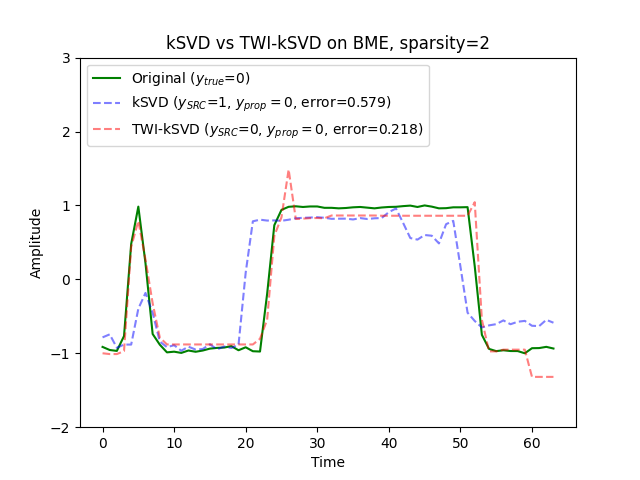
\includegraphics[width=\textwidth]{../../figures/1D_example_sparsity_2.png}
        \caption*{Sparsity = 2}
    \end{subfigure}
    \begin{subfigure}[b]{0.33\textwidth}
        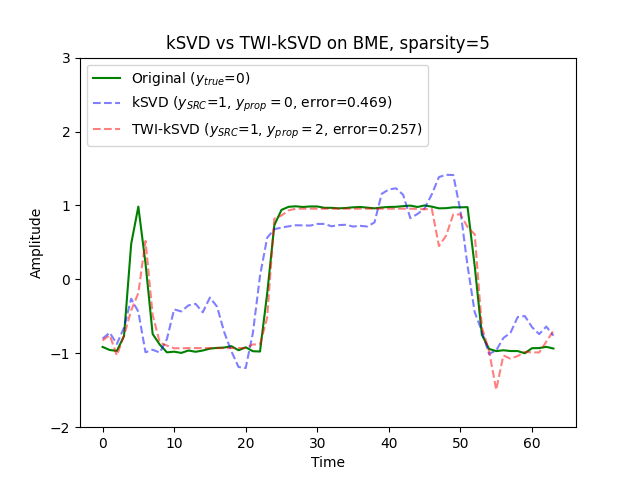
\includegraphics[width=\textwidth]{../../figures/1D_example_sparsity_5.png}
        \caption*{Sparsity = 5}
    \end{subfigure}
    \begin{subfigure}[b]{0.33\textwidth}
        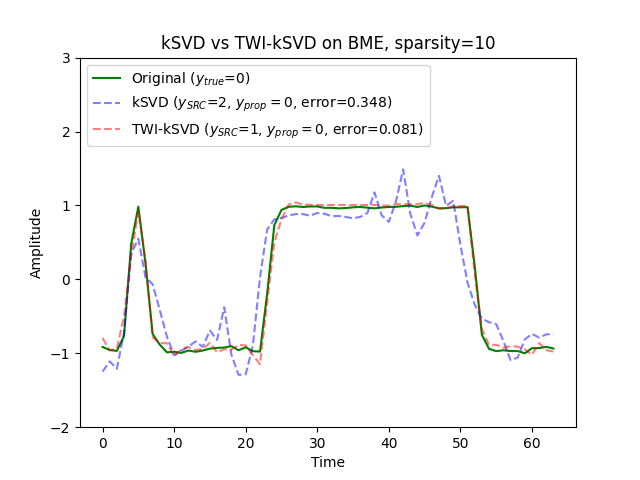
\includegraphics[width=\textwidth]{../../figures/1D_example_sparsity_10.png}
        \caption*{Sparsity = 10}
    \end{subfigure}
    \caption{Example of reconstructions (BME dataset) with different sparsity levels}\label{tab:1D_example}
\end{figure*}


\begin{figure*}[!ht]
    \centering
    \begin{subfigure}[b]{0.49\textwidth}
      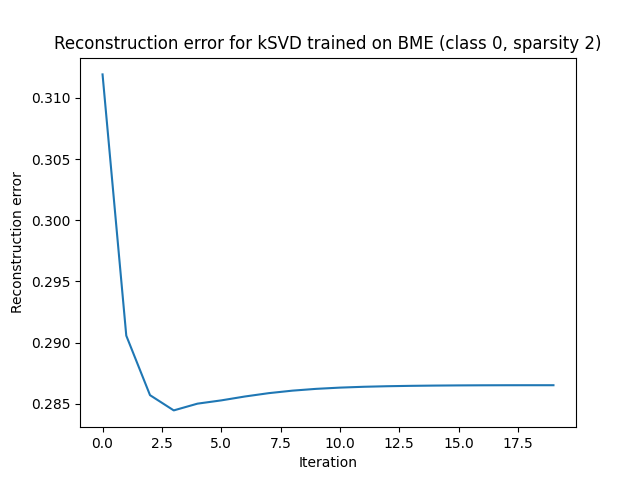
\includegraphics[width=\textwidth]{../../figures/loss_kSVD_spars_2_class_0_BME.png}
      \caption{kSVD}
    \end{subfigure}
    \begin{subfigure}[b]{0.49\textwidth}
        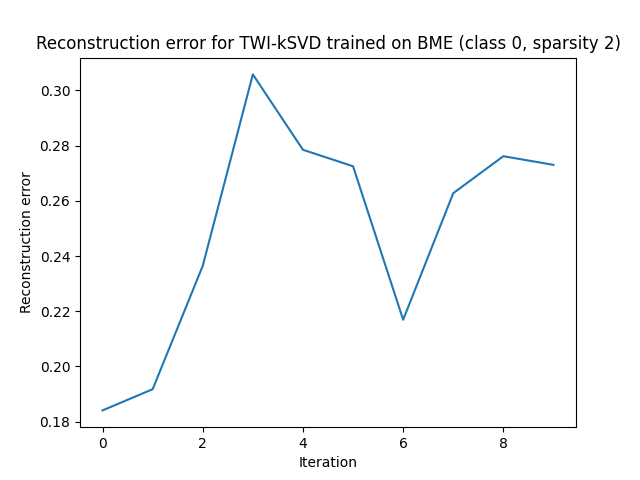
\includegraphics[width=\textwidth]{../../figures/loss_TWI_kSVD_spars_2_class_0_BME.png}
        \caption{TWI-kSVD}
      \end{subfigure}
    \caption{Evolution of reconstruction loss during training (BME dataset)}\label{fig:loss_BME}
\end{figure*}


\begin{figure*}[!ht]
    \centering
    \begin{subfigure}[b]{0.49\textwidth}
      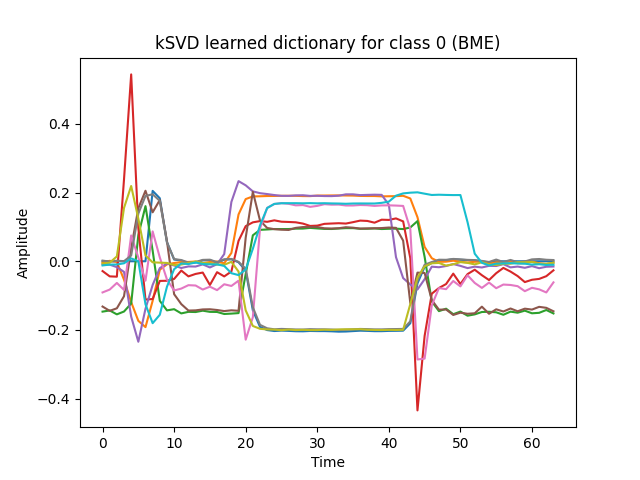
\includegraphics[width=\textwidth]{../../figures/kSVD_dictionary_BME_class_0.png}
      \caption*{kSVD}
    \end{subfigure}
    \begin{subfigure}[b]{0.49\textwidth}
        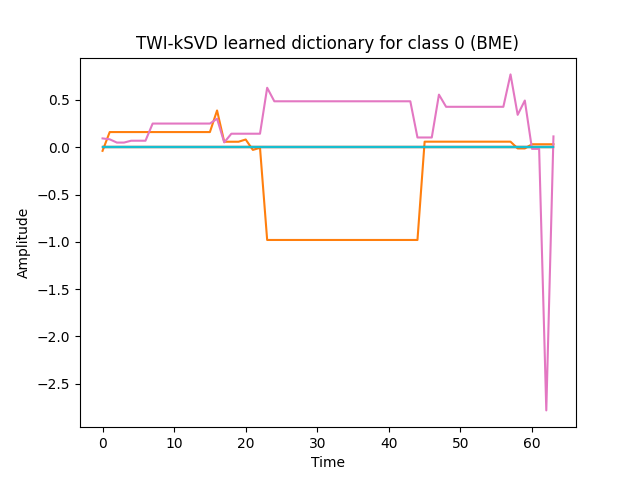
\includegraphics[width=\textwidth]{../../figures/TWI_kSVD_dictionary_BME_class_0.png}
        \caption*{TWI-kSVD}
      \end{subfigure}
    \caption{Learned dictionaries for first class of BME dataset}\label{fig:learn_dicts_BME}
\end{figure*}


\begin{figure*}[!ht]
    \centering
    \begin{subfigure}[t]{\textwidth}
        \centering
        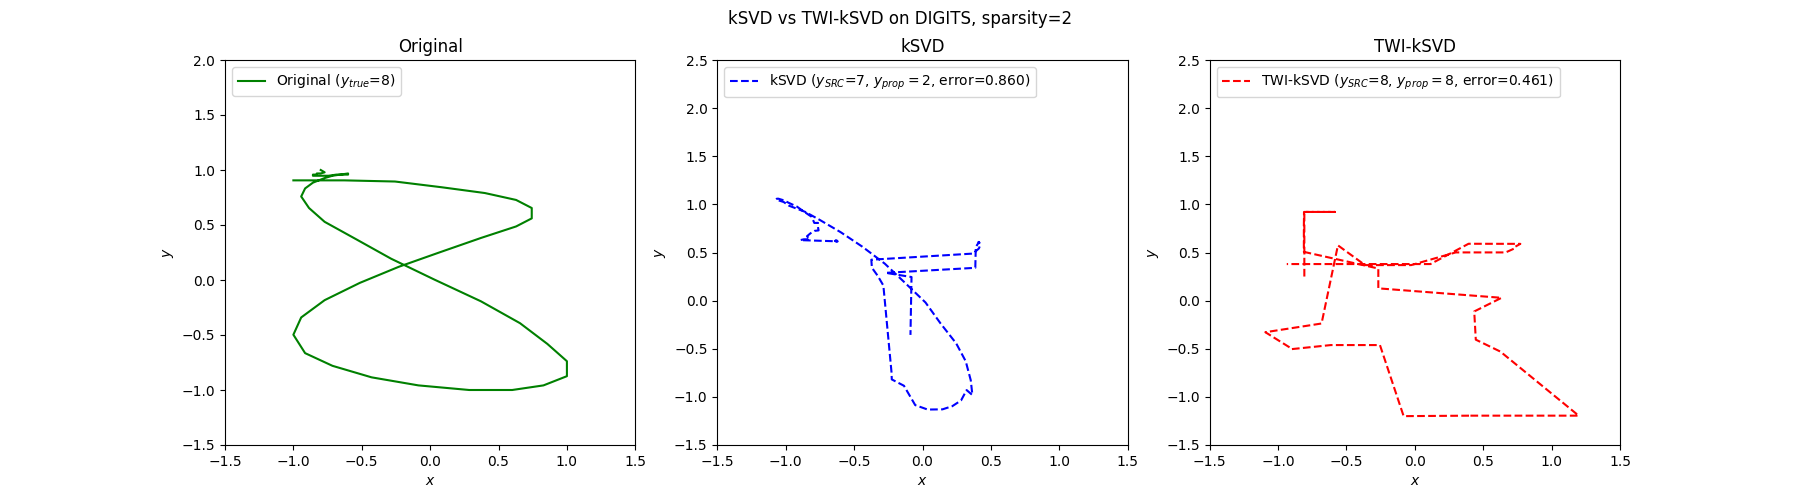
\includegraphics[width=\textwidth]{../../figures/2D_example_sparsity_2.png}
        \caption*{Sparsity = 2}
    \end{subfigure}
    
    \begin{subfigure}[t]{\textwidth}
        \centering
        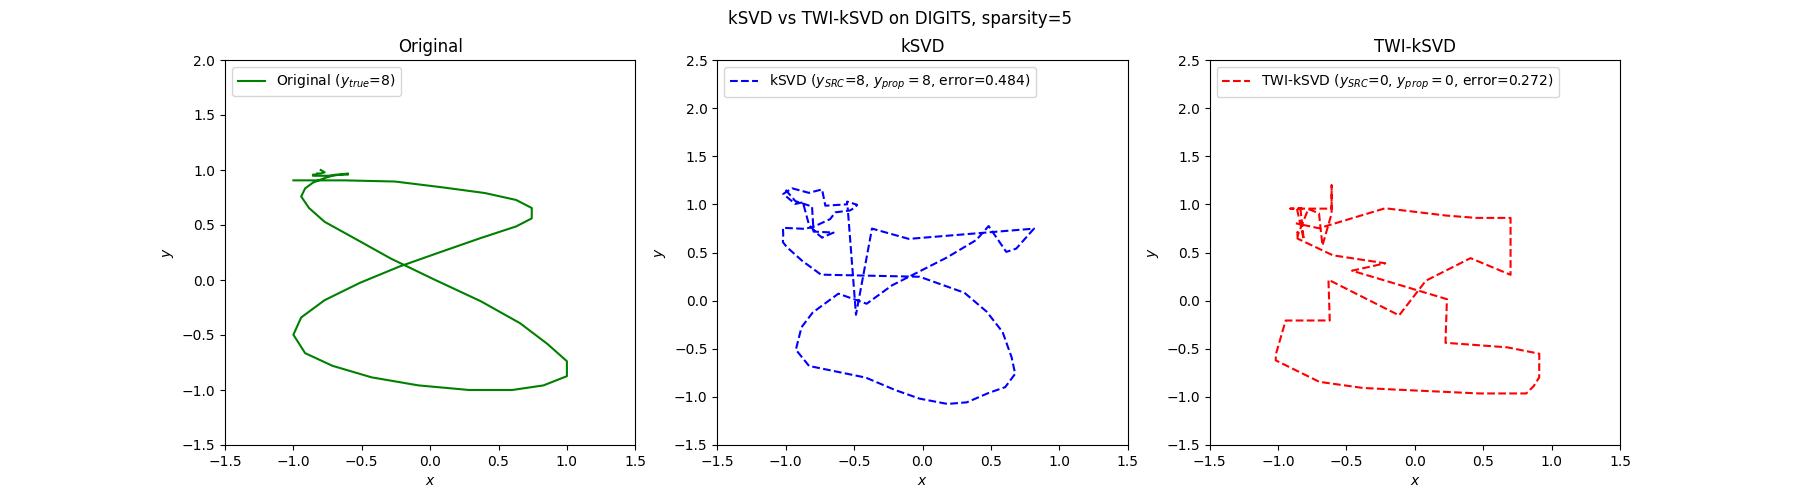
\includegraphics[width=\textwidth]{../../figures/2D_example_sparsity_5.png}
        \caption*{Sparsity = 5}
    \end{subfigure}

    \begin{subfigure}[t]{\textwidth}
        \centering
        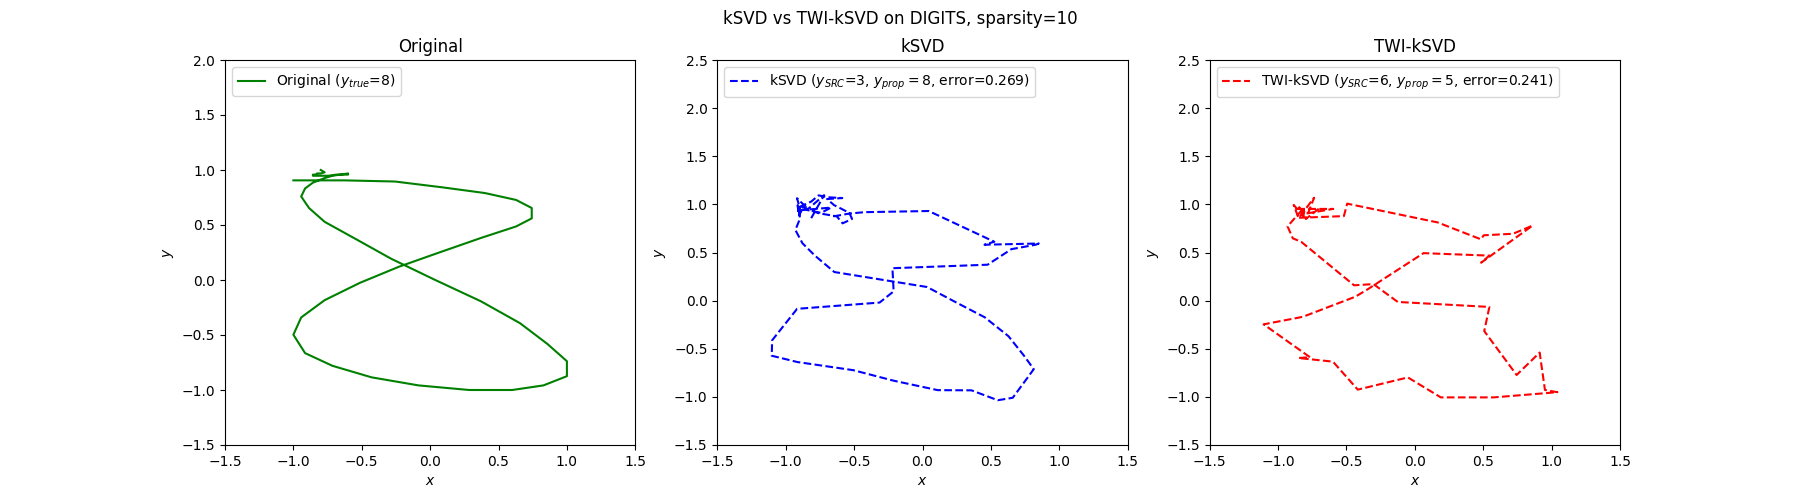
\includegraphics[width=\textwidth]{../../figures/2D_example_sparsity_10.png}
        \caption*{Sparsity = 10}
    \end{subfigure}
        \caption{Example of reconstructions (DIGITS dataset) with different sparsity levels}\label{tab:2D_example}
\end{figure*}


\begin{figure*}[!ht]
    \centering
    \begin{subfigure}[b]{0.49\textwidth}
      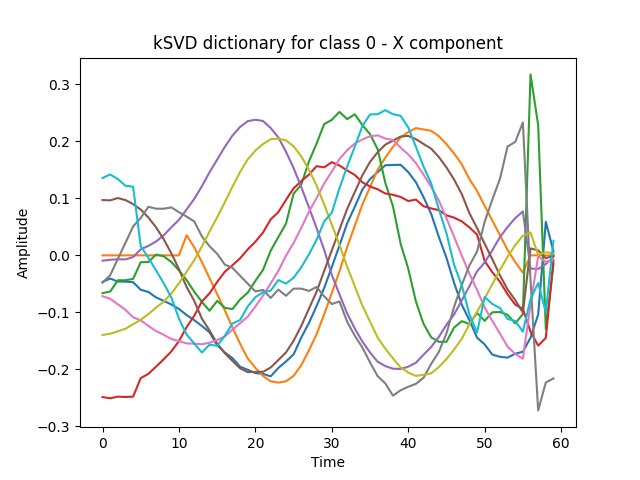
\includegraphics[width=\textwidth]{../../figures/kSVD_dictionnary_DIGITS_class_0_X.png}
      \caption*{kSVD - X component}
    \end{subfigure}
    \begin{subfigure}[b]{0.49\textwidth}
        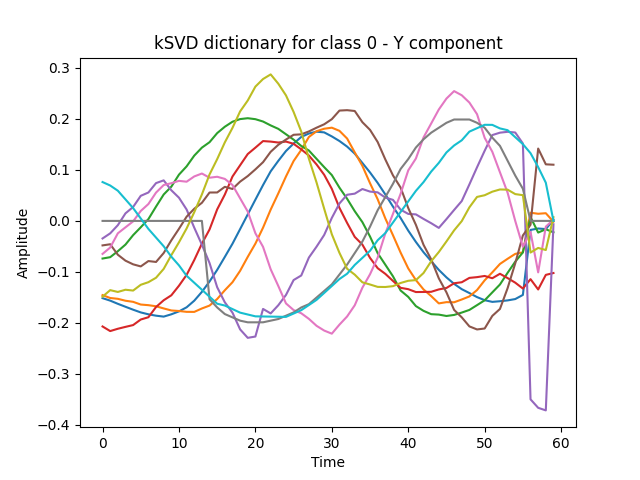
\includegraphics[width=\textwidth]{../../figures/kSVD_dictionnary_DIGITS_class_0_Y.png}
        \caption*{kSVD - Y component}
      \end{subfigure}

      \begin{subfigure}[b]{0.49\textwidth}
        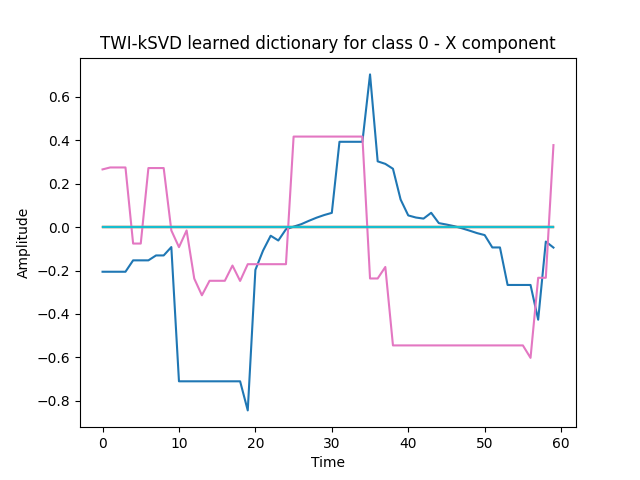
\includegraphics[width=\textwidth]{../../figures/TWI_kSVD_dictionnary_DIGITS_class_0_X.png}
        \caption*{TWI-kSVD - X component}
      \end{subfigure}
      \begin{subfigure}[b]{0.49\textwidth}
          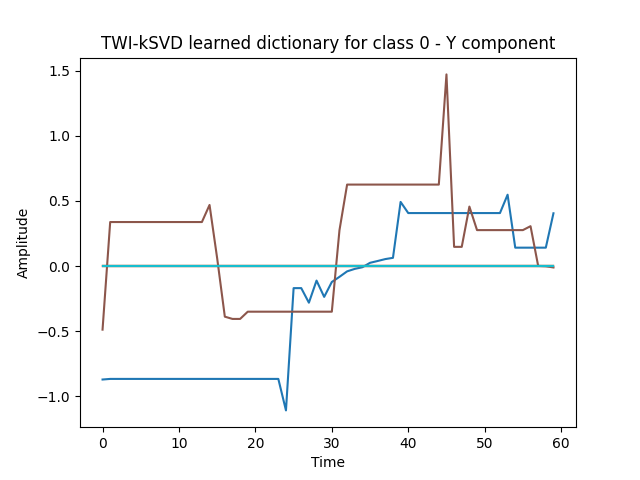
\includegraphics[width=\textwidth]{../../figures/TWI_kSVD_dictionnary_DIGITS_class_0_Y.png}
          \caption*{TWI-kSVD - Y component}
        \end{subfigure}
    \caption{Learned dictionaries for first class of DIGITS dataset}\label{fig:learn_dicts_DIGITS}
\end{figure*}


\begin{figure*}[!ht]
    \centering
    \begin{subfigure}[b]{\textwidth}
      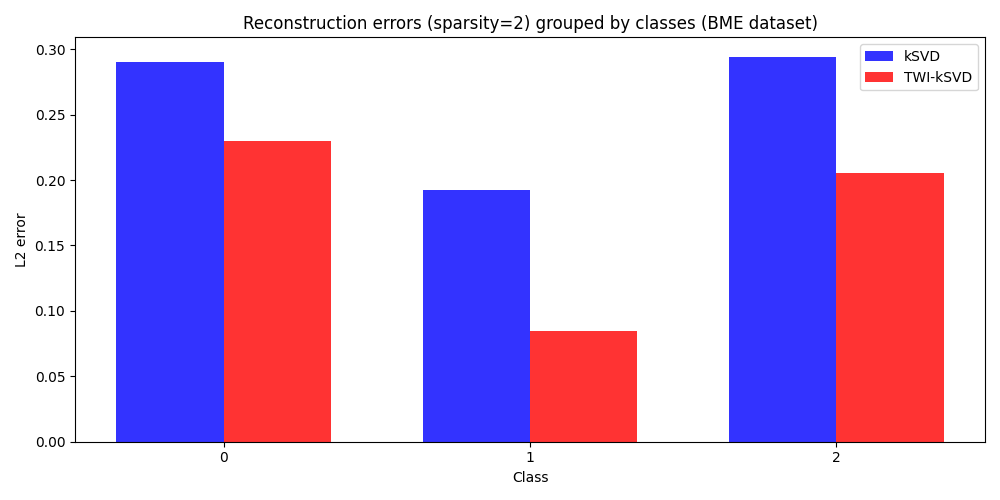
\includegraphics[width=\textwidth]{../../figures/class_barplot_BME_2.png}
      \caption*{BME}
    \end{subfigure}

    \begin{subfigure}[b]{\textwidth}
        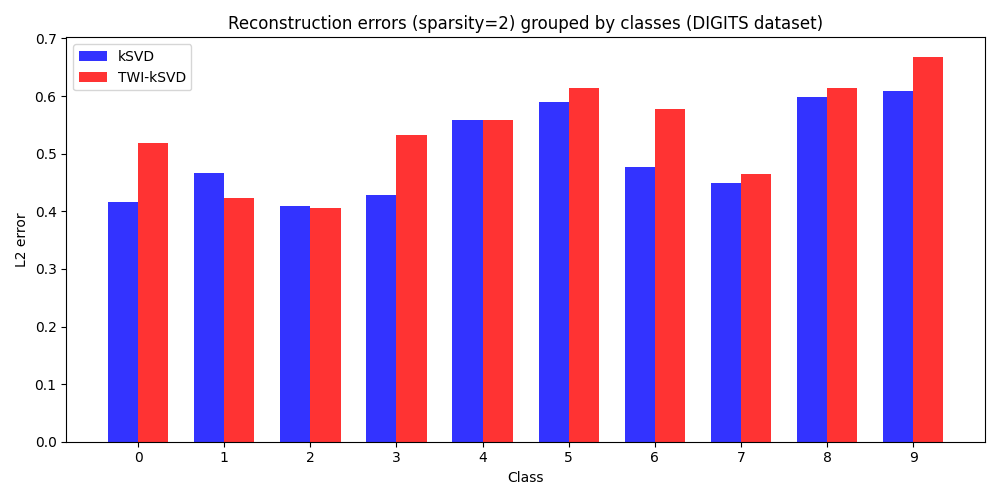
\includegraphics[width=\textwidth]{../../figures/class_barplot_DIGITS_2.png}
        \caption*{DIGITS}
      \end{subfigure}
    \caption{Reconstruction errors grouped by class (both datasets, sparsity = 2)}\label{fig:barplots}
\end{figure*}

\end{document}
